\documentclass[aspectratio=169]{beamer}
\usepackage{tikz}
\usetikzlibrary{arrows,shapes}
\tikzstyle{vertex}=[circle,fill=black!25,minimum size=10pt,inner sep=0pt]
\tikzstyle{blue vertex}=[circle,fill=blue!100,minimum size=10pt,inner sep=0pt]
\tikzstyle{red vertex}=[circle,fill=red!100,minimum size=10pt,inner sep=0pt]
%\tikzstyle{label}=[thin, draw=black, align=center,minimum width=0.5cm, minimum height=0.5cm,fill=white]
\tikzstyle{edge} = [draw,thick,-]
\tikzstyle{red edge} = [draw, line width=5pt,-,red!50]
\tikzstyle{black edge} = [draw, line width=5pt,-,black!20]
\tikzstyle{weight} = [font=\smaller]


\usepackage{amssymb,amsmath}
\usepackage{graphicx}
\usepackage{url}
\usepackage{color}
\usepackage{relsize}		% For \smaller
\usepackage{url}			% For \url
\usepackage{epstopdf}	% Included EPS files automatically converted to PDF to include with pdflatex
\usepackage{pagenote}[continuous,page]

%For MindMaps
% \usepackage{tikz}%
% \usetikzlibrary{mindmap,trees,arrows}%

%%% Color Definitions %%%%%%%%%%%%%%%%%%%%%%%%%%%%%%%%%%%%%%%%%%%%%%%%%%%%%%%%%
%\definecolor{bordercol}{RGB}{40,40,40}
%\definecolor{headercol1}{RGB}{186,215,230}
%\definecolor{headercol2}{RGB}{80,80,80}
%\definecolor{headerfontcol}{RGB}{0,0,0}
%\definecolor{boxcolor}{RGB}{186,215,230}

%%% Save space in lists. Use this after the opening of the list %%%%%%%%%%%%%%%%
%\newcommand{\compresslist}{
%	\setlength{\itemsep}{1pt}
%	\setlength{\parskip}{0pt}
%	\setlength{\parsep}{0pt}
%}

%\setbeameroption{show notes on top}

% You should run 'pdflatex' TWICE, because of TOC issues.

% Rename this file.  A common temptation for first-time slide makers
% is to name it something like ``my_talk.tex'' or
% ``john_doe_talk.tex'' or even ``discrete_math_seminar_talk.tex''.
% You really won't like any of these titles the second time you give a
% talk.  Try naming your tex file something more descriptive, like
% ``riemann_hypothesis_short_proof_talk.tex''.  Even better (in case
% you recycle 99% of a talk, but still want to change a little, and
% retain copies of each), how about
% ``riemann_hypothesis_short_proof_MIT-Colloquium.2000-01-01.tex''?

\mode<presentation>
{
  % A tip: pick a theme you like first, and THEN modify the color theme, and then add math content.
  % Warsaw is the theme selected by default in Beamer's installation sample files.

  %%%%%%%%%%%%%%%%%%%%%%%%%%%% THEME
  %\usetheme{Madrid}		% No subsection
  \usetheme{AnnArbor}  % Subsection on top, no color


  %\usetheme{Antibes}
  %\usetheme{Bergen}
  %\usetheme{Berkeley}		% bem bacana - menu esquerdo
  %\usetheme{Berlin}
  %\usetheme{Boadilla}
  %\usetheme{boxes}
  %\usetheme{CambridgeUS}		% bem bacana - menu superior
  %\usetheme{Copenhagen}
  %\usetheme{Darmstadt}
  %\usetheme{default}
  %\usetheme{Dresden}
  %\usetheme{Frankfurt}
  %\usetheme{Goettingen}
  %\usetheme{Hannover}		% bem bacana - menu esquerdo
  %\usetheme{Ilmenau}
  %\usetheme{JuanLesPins}
  %\usetheme{Luebeck}
  %\usetheme{Malmoe}
  %\usetheme{Marburg}		% bem bacana - menu direito
  %\usetheme{Montpellier}
  %\usetheme{PaloAlto}		% bem bacana - menu esquerdo
  %\usetheme{Pittsburgh}
  %\usetheme{Rochester}		%bacana
  %\usetheme{Singapore}
  %\usetheme{Szeged}
  %\usetheme{Warsaw}

  %%%%%%%%%%%%%%%%%%%%%%%%%%%% COLOR THEME
  %\usecolortheme{default}		% branco, azul clarinho
  \usecolortheme{crane}		% Very yellow (ok)

  %\usecolortheme{albatross}		% azul escuro, massa
  %\usecolortheme{beetle}		% cinza, menu azul
  %\usecolortheme{dolphin}		% azul e branco, legal
  %\usecolortheme{dove}			% cinza e branco, feio
  %\usecolortheme{fly}			% todo cinza, horrível
  %\usecolortheme{lily}			% parece o default
  %\usecolortheme{orchid}		% azul e branco, ok
  %\usecolortheme{rose}			% branco e violeta-claro, bonito
  %\usecolortheme{seagull}		% cinza, feio
  %\usecolortheme{seahorse}		% nhé, meio feio
  %\usecolortheme{sidebartab}		% Azul, branco, destaque na tab, interessante
  %\usecolortheme{structure}		% bichado
  %\usecolortheme{whale}		% Azul e branco, bem bonito

  %%%%%%%%%%%%%%%%%%%%%%%%%%%% OUTER THEME
  \useoutertheme{default}
  %\useoutertheme{infolines}
  %\useoutertheme{miniframes}
  %\useoutertheme{shadow}
  %\useoutertheme{sidebar}
  %\useoutertheme{smoothbars}
  %\useoutertheme{smoothtree}
  %\useoutertheme{split}
  %\useoutertheme{tree}

  %%%%%%%%%%%%%%%%%%%%%%%%%%%% INNER THEME
  \useinnertheme{circles}
  %\useinnertheme{default}
  %\useinnertheme{inmargin}
  %\useinnertheme{rectangles}
  %\useinnertheme{rounded}

  %%%%%%%%%%%%%%%%%%%%%%%%%%%%%%%%%%%

  \setbeamercovered{invisible} % or whatever (possibly just delete it)
  % To change behavior of \uncover from graying out to totally
  % invisible, can change \setbeamercovered to invisible instead of
  % transparent. apparently there are also 'dynamic' modes that make
  % the amount of graying depend on how long it'll take until the
  % thing is uncovered.

}


% Get rid of nav bar
\beamertemplatenavigationsymbolsempty

% Use short top
%\usepackage[headheight=12pt,footheight=12pt]{beamerthemeboxes}
%\addheadboxtemplate{\color{black}}{
%\hskip0.5cm
%\color{white}
%\insertshortauthor \ \ \ \
%\insertframenumber \ \ \ \ \ \ \
%\insertsection \ \ \ \ \ \ \ \ \ \ \ \ \ \ \ \ \  \insertsubsection
%\hskip0.5cm}
%\addheadboxtemplate{\color{black}}{
%\color{white}
%\ \ \ \
%\insertsection
%}
%\addheadboxtemplate{\color{black}}{
%\color{white}
%\ \ \ \
%\insertsubsection
%}

% Insert frame number at bottom of the page.
% \usefoottemplate{\hfil\tiny{\color{black!90}\insertframenumber}}

%% makes the ppagenote command for figure references at the end.

\usepackage[english]{babel}
%qq\usepackage[latin1]{inputenc}
\usepackage{CJKutf8}
\usepackage{subfigure}

\usepackage{times}
\usepackage[T1]{fontenc}

\makepagenote
\renewcommand{\notenumintext}[1]{}
\newcommand{\ppagenote}[1]{\pagenote[Page \insertframenumber]{#1}}

\title[Programming Challenges]{GB20602 - Programming Challenges}
\author[Claus Aranha]{Claus Aranha\\{\footnotesize caranha@cs.tsukuba.ac.jp}}
\institute[U. Tsukuba]{University of Tsukuba, Department of Computer Sciences}


\subtitle[Week 6: Graph II]{Week 6 - Graph Part II: Minimum Path}
\date[]{{\smaller(last updated: \today)}}

\begin{document}
\begin{CJK}{UTF8}{ipxm}

\begin{frame}
\maketitle
\vfill

\hfill Version 2021.1
\end{frame}


\section{Introduction}

\begin{frame}
  \frametitle{Computational Geometry}
  \framesubtitle{What is it?}

  {\small

    \structure{Computational Geometry} problems involve answering
    questions about \structure{lines, points and angles}. Some example
    questions:

    \bigskip

    \begin{block}{}
    \only<1>{Given $N$ points $(s_1, s_2, s_3, \ldots, s_N)$, what is
      the area of the poligon that covers all the points?}

    \only<2>{Given $N$ rectangles, $x_1,y_1,w_1,h_1; \ldots; x_N, y_N,
      w_N, h_N$, what is the length of lines needed to connect them?}

    \only<3>{Given a polygon, and $N$ points, what is the line
      that divides the polygon in equal areas, so that the same
      number of points are in each area?}
    \end{block}

    \begin{center}
      \includegraphics<1>[width=0.8\textwidth]{img/sampleproblem_1.png}
      \includegraphics<2>[width=0.6\textwidth]{img/sampleproblem_2.png}
      \includegraphics<3>[width=0.4\textwidth]{img/sampleproblem_3.png}
    \end{center}

  }
\end{frame}

\begin{frame}
  \frametitle{Computational Geometry}
  \framesubtitle{The good and the bad}

  \begin{itemize}
  \item \structure{Good}: Geometry problems are fun
  \item \structure{Good}: You have to draw pretty pictures
  \item \structure{Good}: Mostly algorithms from high school
  \item \structure{Good}: Code is highly re-usable

    \bigskip

  \item \alert{Bad}: You have to write a lot of code (in the beginning!)
  \item \alert{Bad}: Very easy to get WE...
  \end{itemize}
\end{frame}


\begin{frame}
  \frametitle{Easy Mistakes in Geometry Problems}

  {\small
    \begin{block}{Problem 1 -- Special Cases}
      \begin{itemize}
      \item Multiple points in the same place;
      \item Collinear points;
      \item Vertical lines;
      \item Parallel Lines;
      \item Intersection at end of segment;
      \item etc;
      \end{itemize}
    \end{block}

    \begin{block}{Problem 2 -- Precision Errors}
      \begin{itemize}
      \item Functions require many multiplications and divisions;
      \item Easy to propagate floating point errors;
      \end{itemize}
    \end{block}
  }
\end{frame}


\begin{frame}[fragile]
  \frametitle{Easy Mistakes in Geometry Problems}

  {\smaller

    \begin{block}{Dealing Special Cases}
      \begin{itemize}
      \item Make sure to add special cases to your
        library functions;
      \end{itemize}
    \end{block}

    \begin{block}{Solving Precision Errors}
      \begin{itemize}
      \item If possible, convert all values to integers
      \item Use an EPSILON constant for comparisons:

\begin{verbatim}
if (float.1 == float.2) then            // NO
if (fabs(float.1 - float.2) < EPS) then // YES!
\end{verbatim}

      \end{itemize}
    \end{block}
  }
\end{frame}

\begin{frame}
  \frametitle{Class Outline}
  \begin{itemize}
  \item Example Problems;
  \item Basic Geometric Functions;
  \item Circles;
  \item Triangles;
  \item Polygons;
  \end{itemize}
\end{frame}

\section{Single Source Shortest Path}

\begin{frame}
  \begin{center}
    {\bf Part I - Single Source Shortest Path}
  \end{center}
\end{frame}

\subsection{Definitions}
\begin{frame}
  \frametitle{SSSP: Single Source Shortest Path}
  \begin{block}{Problem Definition}
    In a graph $G(V,E)$, find the path from vertec $v_s$ (source) to vertex $v_t$ (target), where {\bf the sum of edge weights is minimal}.
  \end{block}\bigskip

  \begin{itemize}
  \item For an {\bf unweighted graph}, we consider the weight of every edge $e_i \in E$ to be equal to one;\medskip

  \item In this case, Breadth First Search (BFS) is actually good enough;\medskip

  \item Start BFS on node $v_s$;\medskip

  \item BFS will visit all nodes in the graph in order of distance, eventually reaching $v_t$ (if it is reachable);
  \end{itemize}
\end{frame}

\begin{frame}[fragile]
  \frametitle{BFS Implementation for SSSP}

{\smaller
\begin{exampleblock}{}
\begin{verbatim}
vector <int> p;                          // parent list
vector <int> dist(V,100*V); dist[s] = 0; // dist matrix
queue  <int> q;           q.push(s);

while (!q.empty()) {
   int u = q.front(); q.pop();
   for (int j = 0; j < AdjList[u].size(); j++) {
      int v = AdjList[u][j];
      if (dist[v] > V) {                 // not visited
         dist[v] = dist[u] + 1;
         p[v] = u; q.push(v); }}}

void printPath(u) {                      // path from (u)
   if (u == s) { cout << s; return; }
   printPath(p[u]); cout << " " << u; }
\end{verbatim}
\end{exampleblock}
}
\end{frame}

\begin{frame}
  \frametitle{BFS: Problem with weighted graphs}

  \begin{block}{}
    The BFS is a simple and fast algorithm. However, if the graph has edge weights, it may give you a Wrong Answer to find the SSSP
  \end{block}

  \medskip

  \begin{center}
    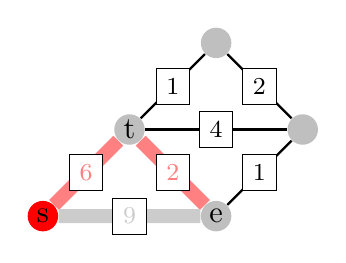
\begin{tikzpicture}[transform shape,label/.style={thin, draw=black, align=center,fill=white,font=\smaller},scale=1.1]
      \node[vertex] (a) at (0,0) {t};
      \node[vertex] (b) at (1,1) {};
      \node[vertex] (c) at (2,0) {};
      \node[vertex] (d) at (1,-1) {e};
      \node[red vertex] (e) at (-1,-1) {s};
      \draw[edge] (a) -- node[label] {$1$} (b);
      \draw[edge] (b) -- node[label] {$2$} (c);
      \draw[edge] (a) -- node[label] {$4$} (c);
      \draw[red edge] (a) -- node[label] {$2$} (d);
      \draw[edge] (c) -- node[label] {$1$} (d);
      \draw[red edge] (a) -- node[label] {$6$} (e);
      \draw[black edge] (d) -- node[label] {$9$} (e);
    \end{tikzpicture}
  \end{center}

  \bigskip

  \begin{itemize}
  \item BFS shortest path: $s \rightarrow e$ (1 edge, cost 9)
  \item Real shortest path: $s \rightarrow t \rightarrow e$ (2 edges, cost 8)
  \end{itemize}
\end{frame}

\subsection{Dijkstra Algorithm}
\begin{frame}
  \frametitle{SSSP on weighted graphs: Dijkstra's Algorithm}
  \begin{block}{Basic Idea:}
    Greedy graph search: Always follow the edge with the {\bf minimal total distance} from the source node.
  \end{block}\bigskip

  \begin{itemize}
  \item There are many different implementations;
  \begin{itemize}
    \item (The original paper did not include an implementation!)
  \end{itemize}\bigskip

  \item Simple implementation: replace the BFS {\bf queue} with a {\bf Priority Queue}:
  \begin{itemize}
    \item The priority queue sorts the edges with minimum total distance;
  \end{itemize}\bigskip

  \item Minor optimization:
  \begin{itemize}
    \item C++ STL priority queue has large cost to deleting/updating edges;
    \item To avoid this cost, we use "lazy deletion" to skip longer paths;
  \end{itemize}
  \end{itemize}

\end{frame}

\begin{frame}[fragile]
  \frametitle{Dijkstra's Algorithm Implementation Example}

  This implementation uses {\bf Lazy Skipping} to reduce the number of deletions from the priority queue;

  {\smaller
    \begin{exampleblock}{}
\begin{verbatim}
typedef pair<int,int> ii;           // <distance, to_vertex>
priority_queue<ii, vector<ii>, greater<ii>> pq;
pq.push({0,s});

while (!pq.empty()) {
  auto [d, u] = pq.top(); pq.pop(); // shortest unvisited u
  if (d > dist[u]) continue;        // **Lazy skipping**
  for (auto &[v, w] : AdjList[u]) { // all edges from u
    if (dist[u] + w >= dist[v]) continue;
       // new edge does not improve solution, skip
    dist[v] = dist[u] + w           // update distance
    pq.push({dist[v], v})           // enqueue better pair
  }
\end{verbatim}
    \end{exampleblock}}
\end{frame}

\begin{frame}[fragile]{Dijkstra with Lazy deletion: Simulation}
  Dijkstra visits vertices: 2, 1, 3, 0, 4; in order
  \begin{columns}[T]
    \column{0.6\textwidth}
    \begin{center}
      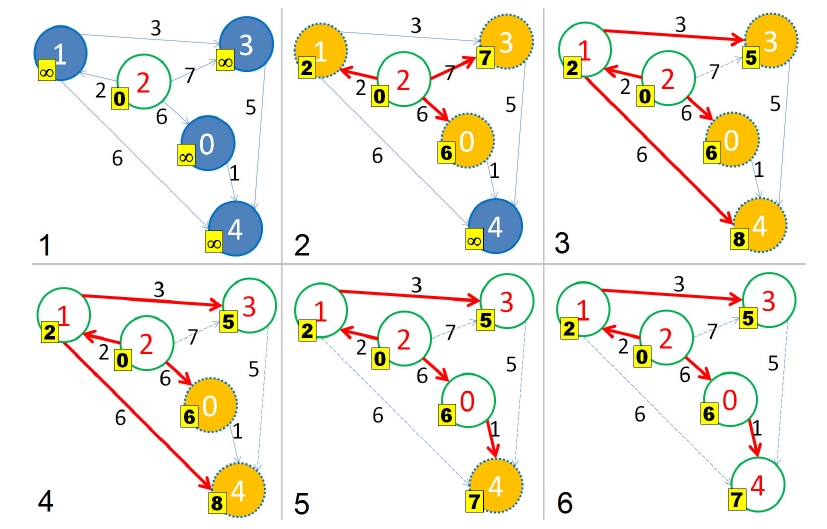
\includegraphics[width=.9\textwidth]{../img/dijkstra_halim}
      \ppagenote{Dijkstra Image from "Competitive Programming 3", Steven Halim}
    \end{center}
    \column{.4\textwidth}
\begin{verbatim}
 PQ:
\end{verbatim}
  \end{columns}
\end{frame}

\subsection{Problem Example}

\begin{frame}{SSSP in Programming Challenges}
  \begin{itemize}
    \item Of course, just giving a graph as input, and asking you to find the SSSP is not a very exciting programming challenge. \bigskip

    \item Because of this, programming challenges will usually require you to {\bf change or build the graph structure} from the input data.\bigskip

    \item Let's see one example;
  \end{itemize}
\end{frame}

\begin{frame}
  \frametitle{UVA 11367 -- Full Tank}
  \begin{block}{Problem Summary}
    Find the {\bf cheapest} path from city $S$ to city $T$. Consider the following:

    \begin{itemize}
      \item To go from $v_i$ to $v_j$ requires $E_{i,j}$ {\bf liters of fuel};
      \item The price of fuel in city $v_i$ is $p_i$;
      \item Your car has maximum capacity $c$;
    \end{itemize}
  \end{block}

  \begin{center}
    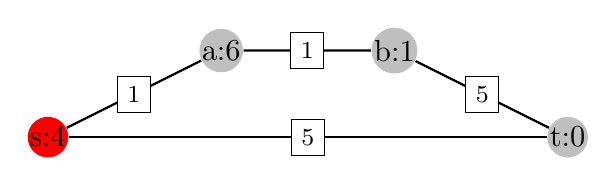
\begin{tikzpicture}[transform shape,label/.style={thin, draw=black, align=center,fill=white,font=\smaller},scale=1.1]
      \node[red vertex] (s) at (0,0) {s:4};
      \node[vertex] (0) at (2,1) {a:6};
      \node[vertex] (1) at (4,1) {b:1};
      \node[vertex] (e) at (6,0) {t:0};
      \draw[edge] (s) -- node[label] {$5$} (e);
      \draw[edge] (s) -- node[label] {$1$} (0);
      \draw[edge] (0) -- node[label] {$1$} (1);
      \draw[edge] (1) -- node[label] {$5$} (e);
    \end{tikzpicture}
  \end{center}

  \begin{itemize}
    \item Path: $s\to t$: Buy 10 liters at $s$, cost: 20
    \item Path: $s\to a\to b\to t$:
    \begin{itemize}
      \item Buy 4 liters at $s$, 10 liters at $b$, cost: 9
    \end{itemize}
    \item {\bf QUIZ}: How to implement SSSP for this one?
  \end{itemize}
\end{frame}

\begin{frame}
  \frametitle{UVA 11367 -- Full Tank: Graph Modification}

    \begin{center}
      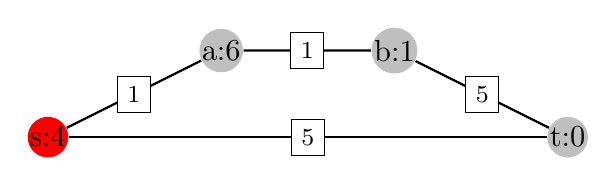
\begin{tikzpicture}[transform shape,label/.style={thin, draw=black, align=center,fill=white,font=\smaller},scale=1.1]
        \node[red vertex] (s) at (0,0) {s:4};
        \node[vertex] (0) at (2,1) {a:6};
        \node[vertex] (1) at (4,1) {b:1};
        \node[vertex] (e) at (6,0) {t:0};
        \draw[edge] (s) -- node[label] {$5$} (e);
        \draw[edge] (s) -- node[label] {$1$} (0);
        \draw[edge] (0) -- node[label] {$1$} (1);
      \draw[edge] (1) -- node[label] {$5$} (e);
      \end{tikzpicture}
    \end{center}

    \begin{itemize}
      \item Transform vertex $v_i$ into a set of vertices $v_{i,f}$: $v_{i,0}, v_{i,1}, \ldots, v_{i,c}$;
      \begin{itemize}
        \item This represents the car at $v_i$ with $f$ fuel left;
      \end{itemize}
      \item An edge exists between $v_{i,k}$ and $v_{i,k+1}$ with cost $p_i$;
      \begin{itemize}
        \item This represents adding fuel to the car.
      \end{itemize}
      \item An edge exists between $v_{i,k}$ and $v_{j,k-w_{i,j}}$ if exits an edge $v_i \to v_k$ with cost $w_{i,j}$ and $k-w_{i,j} \geq 0$;
      \begin{itemize}
        \item This represents the car has enough fuel to go to j
      \end{itemize}
      \item Now we can do Dijkstra in the modified graph;
      \item Note the new graph has $V\times C$ vertices and $E\times C$ edges;
    \end{itemize}
\end{frame}

\begin{frame}
  \frametitle{UVA 11367 -- Full Tank: Simulation of Graph Transformation}

    \begin{center}
      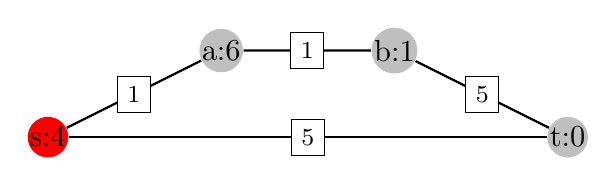
\begin{tikzpicture}[transform shape,label/.style={thin, draw=black, align=center,fill=white,font=\smaller},scale=1.1]
        \node[red vertex] (s) at (0,0) {s:4};
        \node[vertex] (0) at (2,1) {a:6};
        \node[vertex] (1) at (4,1) {b:1};
        \node[vertex] (e) at (6,0) {t:0};
        \draw[edge] (s) -- node[label] {$5$} (e);
        \draw[edge] (s) -- node[label] {$1$} (0);
        \draw[edge] (0) -- node[label] {$1$} (1);
      \draw[edge] (1) -- node[label] {$5$} (e);
      \end{tikzpicture}
    \end{center}
    \vspace{10cm}

\end{frame}

\subsection{Negative Loops}
\begin{frame}
  \frametitle{A Problem with Dijkstra}

    \begin{block}{}
      The dijkstra implementation that we discussed will fall into an {\bf infinite loop} if the graph includes a {\bf negative loop}!
    \end{block}

    \begin{center}
      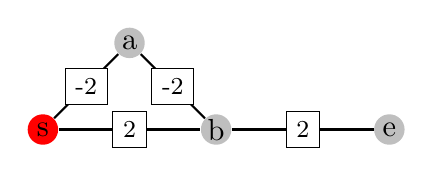
\begin{tikzpicture}[transform shape,label/.style={thin, draw=black, align=center,fill=white,font=\smaller},scale=1.1]
        \node[red vertex] (s) at (0,0) {s};
        \node[vertex] (0) at (1,1) {a};
        \node[vertex] (1) at (2,0) {b};
        \node[vertex] (e) at (4,0) {e};
        \draw[edge] (s) -- node[label] {-2} (0);
        \draw[edge] (s) -- node[label] {2} (1);
        \draw[edge] (1) -- node[label] {-2} (0);
      \draw[edge] (1) -- node[label] {2} (e);
      \end{tikzpicture}
    \end{center}

    \begin{itemize}
    \item Our Dijkstra implementation will add smaller and smaller costs to the priority queue:
    \begin{itemize}
      \item $s \to a$: -2, -4, -6, -8...
    \end{itemize}

    \item We could try to check for used edges; but that will not {\bf detect} negative loops;

    \item {\bf Bellman Ford's algorithm} is a simple SSSP algorithm that can {\bf detect negative loops};
    \end{itemize}
\end{frame}

\begin{frame}[fragile]
  \frametitle{Bellman Ford's Algorithm -- ($O(VE)$)}
  {\smaller
  \begin{itemize}
    \item The main idea is to propagate the weight of every edge $i\to j$, $V-1$ times.

    \item The vector of distances from $s$, \emph{dist}, starts with dist[s]=0, and dist[!s]=INF;

    \item Each iteration, non-inf values of dist propagate;

    \item Because the algorithm has a finite number of loops, it always terminates;
    \item Algorithm stabilizes at iteration $V-1$. If dist changes after that, we have detected an infinite loop.
  \end{itemize}

  \begin{exampleblock}{Pseudocode (uses EdgeList data structure)}
\begin{verbatim}
vector<int> dist(V, INF); dist[s] = 0;  // Start Condition
int edges[E][3];                        // Edge list (i,j,w)
for (int i = 0; i < V - 1; i++)         // repeat V-1 times
 for (int u = 0; u < E; u++) {          // for all edges
  dist[edges[u][1]] = min(dist[edges[u][1]],
                          dist[edges[u][0]]+edges[u][2]);
 }
\end{verbatim}
\end{exampleblock}}
\end{frame}

\begin{frame}
  \frametitle{Bellman Ford Simulation: Regular Graph}
  \begin{center}
    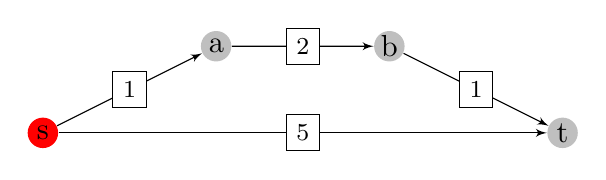
\begin{tikzpicture}[transform shape,label/.style={thin, draw=black, align=center,fill=white,font=\smaller},scale=1.1]
      \node[red vertex] (s) at (0,0) {s};
      \node[vertex] (0) at (2,1) {a};
      \node[vertex] (1) at (4,1) {b};
      \node[vertex] (e) at (6,0) {t};
      \tikzset{edge/.style = {->, >=latex'}}
      \draw[edge] (s) to node[label] {$5$} (e);
      \draw[edge] (s) to node[label] {$1$} (0);
      \draw[edge] (0) to node[label] {$2$} (1);
      \draw[edge] (1) to node[label] {$1$} (e);
    \end{tikzpicture}
  \end{center}
  \vspace{10cm}
\end{frame}

\begin{frame}
  \frametitle{Bellman Ford Simulation: Negative Loop}
  \begin{center}
    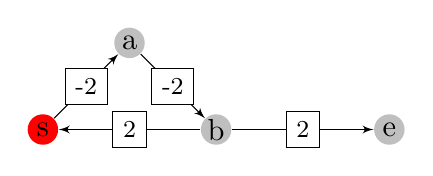
\begin{tikzpicture}[transform shape,label/.style={thin, draw=black, align=center,fill=white,font=\smaller},scale=1.1]
      \node[red vertex] (s) at (0,0) {s};
      \node[vertex] (0) at (1,1) {a};
      \node[vertex] (1) at (2,0) {b};
      \node[vertex] (e) at (4,0) {e};
      \tikzset{edge/.style = {->, >=latex'}}
      \draw[edge] (s) to node[label] {-2} (0);
      \draw[edge] (1) to node[label] {2} (s);
      \draw[edge] (0) to node[label] {-2} (1);
    \draw[edge] (1) to node[label] {2} (e);
    \end{tikzpicture}
  \end{center}
  \vspace{10cm}
\end{frame}

\subsection{}
\begin{frame}
  \frametitle{SSSP Summary}
  \begin{itemize}
  \item \structure{BFS}: $O(V+E)$, only for unweighted graphs;\bigskip

  \item \structure{Dijkstra}: $O(E+V\text{log}V)$, not guaranteed to stop if there is a negative loop;\bigskip

  \item \structure{Bellman Ford}: $O(EV)$ guaranteed to stop;
  \end{itemize}
  \bigskip

  Be familiar with all of them, and use the most appropriate one (or simplest one) for each problem!
\end{frame}


\section{APSP}

\begin{frame}
  \begin{center}
    {\bf Part II -- All Parts Shortest Paths}
  \end{center}
\end{frame}

\subsection{All Pairs Shortest Path}
\begin{frame}
  \frametitle{APSP: All Pairs Shortest Path}

  Consider the following problem:

  \begin{block}{UVA 11463 -- Commandos}
    Consider a graph $G(V,E)$, with a starting vertex $v_s$ and an end vertex $v_t$. You must send a group of commands to visit every vertex in the graph.\bigskip

    Calculate the minimum time to complete all visits, if you can send the commandos in parallel.
  \end{block}

  {\bf Quiz:} How do you solve this problem?
\end{frame}

\begin{frame}{APSP: Commandos Problem}
  \begin{itemize}
  \item To solve this problem, you need to calculate, for every vertex, the shortest path from $v_s$ to $v_t$ that includes that vertex; The solution is the largest of these paths.\bigskip

  \item One simple way to program this is to loop through all vertices $v_i$, and calculate Dijkstra$(v_s,v_i)$ + Dijkstra$(v_i,v_t$);
  \begin{itemize}
    \item The cost would be about $O(V(E+V))$;
  \end{itemize}\bigskip

  \item Let's introduce a {\bf simpler} (but not cheaper!) way to write this program.
  \end{itemize}
\end{frame}

\begin{frame}[fragile]{The Floyd-Warshall Algorithm -- $O(V^3)$}{Only four lines of code!}

  \begin{exampleblock}{}
\begin{verbatim}
int AdjMat[V][V]; // Adjacency Matrix
// Initialization: AdjMat[i][j] contains cost
// of i->j edge, or INF if no edge.

for (int k=0; k < V; k++) // loop order
  for (int i=0; i < V; i++)
    for (int j=0; j < V; j++)
      AdjMat[i][j] = min(AdjMat[i][j],
                         AdjMat[i][k]+AdjMat[k][j]);

// AdjMat[i][j]: cost of minimum path i -> j
\end{verbatim}
  \end{exampleblock}

  \begin{itemize}
  \item Algorithm is slower! So only use it on small graphs;
  \item Very easy to program: Fewer bugs!
  \end{itemize}
\end{frame}

\begin{frame}
  \frametitle{How does Floyd Warshall work?}

  \begin{block}{}
    \begin{itemize}
      \item The basic idea of FW, is Bottom-up dynamic programming;
      \item For every vertex $v_k$, the shortest path between $v_i$ and $v_j$ is either:
      \begin{itemize}
        \item The current shortest path $v_i \to v_j$ or;
        \item The new shortest path $v_i \to v_k \to v_j$;
      \end{itemize}
      \item Every iteration $k$, FW adds $v_k$ to all other existing paths.
    \end{itemize}
  \end{block}

  \begin{center}
    \includegraphics<1>[height=0.5\textheight]{../img/fw_halim1}
    \includegraphics<2>[height=0.5\textheight]{../img/fw_halim2}
    \includegraphics<3>[height=0.5\textheight]{../img/fw_halim3}
    \includegraphics<4>[height=0.5\textheight]{../img/fw_halim4}
  \end{center}
  \ppagenote{Floyd-Warshall Image from "Competitive Programming", Steven Halim}
\end{frame}

\begin{frame}[fragile]{Getting more from Floyd Warshall -- 1}
  \begin{block}{I want to print the shortest path from Floyd Warshall}
To print the shortest path in FW, we add a 2D matrix $p$, where $p[i][j]$ is the last node on the shortest path from i to j
{\smaller
\begin{verbatim}
// Initialize parent matrix
for (int i = 0; i < V; i++)
  for (int j = 0; j < V; j++)
    p[i][j] = i;

// Floyd Warshall
for (int k = 0; k < V; k++)
  for (int i = 0; i < V; i++)
    for (int j = 0; j < v; j++)
      if (AdjMat[i][k] + AdjMat[k][j] < AdjMat[i][j]) {
        AdjMat[i][j] = AdjMat[i][k] + AdjMat[k][j];
        p[i][j] = p[k][j];      // Update parent Matrix
      }
\end{verbatim}}
  \end{block}
\end{frame}


\begin{frame}[fragile]{Getting more from Floyd Warshall -- 2}

  \begin{itemize}
  \item If we only want to know if $v_i$ is connected to $v_j$, we can use FW with bitwise operations -- much faster:
  \begin{verbatim}
  AdjMat[i][j] |= AdjMat[i][k] && AdjMat[k][j];
  \end{verbatim}

  \item We can use FW instead of MST to find the minmax path:
  {\smaller\begin{verbatim}
AdjMat[i][j]=min(AdjMat[i][j],max(AdjMat[i][k],AdjMat[k][j]);
\end{verbatim}}\medskip

  \item We can use FW to find SCCs:
  \begin{itemize}
    \item If AdjMat[i][j] $> 0$ AND AdjMat[j][i] $> 0$, $v_i$ and $v_j$ are in same SCC;
  \end{itemize}\medskip

  \item Use FW to detect negative cycles (or minimum cycles):
  \begin{itemize}
    \item for $i = 0\to V$, check AdjMat[i][i];
    \item If negative: negative loop;
    \item Else: minimum loop.
  \end{itemize}
  \end{itemize}
\end{frame}

\section{Network Flow}

\begin{frame}
  \begin{center}
    {\bf Part III - Network Max Flow}
  \end{center}
\end{frame}

\begin{frame}
  \frametitle{Network Max Flow -- Problem Definition}

  \begin{block}{}
    Consider a {\bf weighted} network of pipes. The weight is the size of each pipe. Water enters the network at $v_s$ and leave at $v_t$. How much water is leaving through $v_t$?
  \end{block}

  \begin{center}
    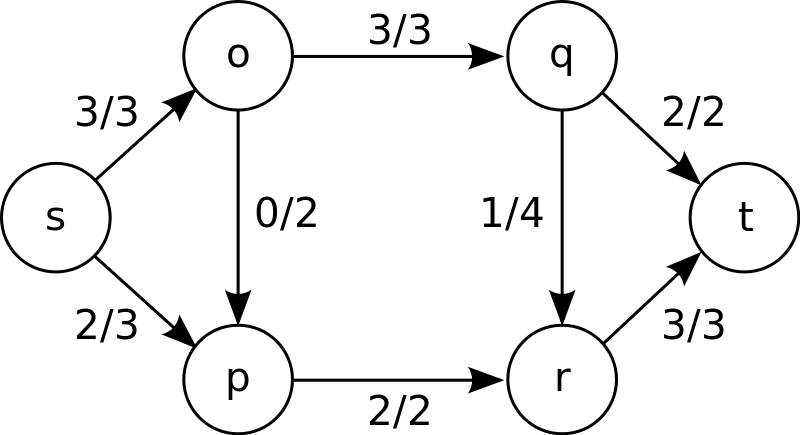
\includegraphics[width=.45\textwidth]{../img/maxflow_wiki}
    \ppagenote{Network Flow Image CC-BY-SA 3.0 by Maksim}
  \end{center}

  \begin{itemize}
    \item 2 units come through $s\to o \to q \to t$,
    \item 2 units come through $s\to p\to r\to t$,
    \item 1 unit comes through $s\to o\to q\to r\to t$.
  \end{itemize}
\end{frame}

\begin{frame}
  \frametitle{Network Max Flow -- Problem Definition}
  \begin{center}
    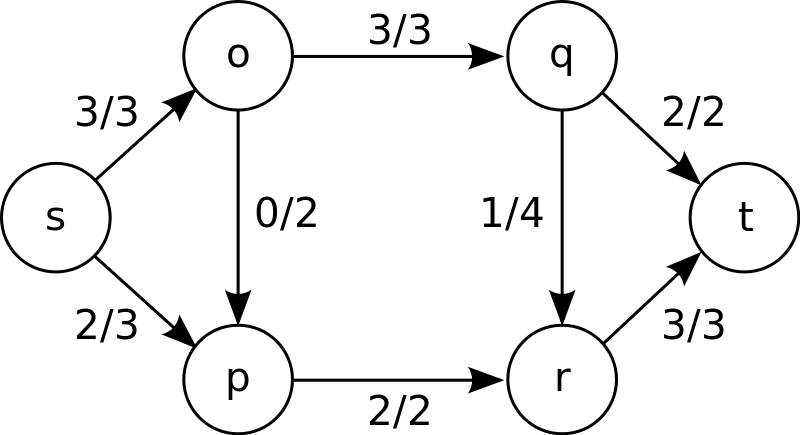
\includegraphics[width=.55\textwidth]{../img/maxflow_wiki}
  \end{center}
  \bigskip

  The goal of the Max Flow problem is to find the maximum total flow that can go between $v_s$ and $v_t$ in a given graph.
\end{frame}


\begin{frame}[fragile]
  \frametitle{Ford Fulkerson Method for Max Flow}

  \begin{block}{}
    The Ford-Fulkerson method\footnote{Same Ford as in Bellman-Ford} finds the maximum flow using a {\bf Residual Flow Graph} to keep track of remaining capacity.
  \end{block}

  \medskip

  \begin{itemize}
  \item {\bf Initialize Residual Graph F}: equal to the original graph G, but directed (add edges as necessary)\medskip
  \item {\bf Main Loop:} If there is a path $p$ between $v_s$ and $v_t$ in F:
  \begin{itemize}
    \item Find smallest weight $w$ in p;
    \item For every edge $E_{u,v} \in p$, {\bf subtract} w from each edge;
    \item For every back-edge $E_{v,u} | E_{u,v}\in p$, {\bf add} w to each edge;
    \item Find another path $v_s \to v_t \in F$
  \end{itemize}
  \end{itemize}
\end{frame}

\begin{frame}[fragile]
  \frametitle{Ford Fulkerson -- Pseudocode}
% {\smaller
  \begin{exampleblock}{}
\begin{verbatim}
int residual[V][V];                   // Initialize Residual Graph
memset(residual, 0, sizeof(residual))
for (int i; i < V; i++)
  for (int j; j < V; j++)
    residual[i][j] = AdjMat[i][j];
mf = 0;                               // Max flow counter
while (P = FindPath(s, t)) {          // Find new path;
   m = P.min_weight;                  // minimum edge in P
   for (edge (v,u) in P) {
      residual[v][u] -= m;
      residual[u][v] += m;
   }
   mf += m;
}
\end{verbatim}
  \end{exampleblock}
  % }
\end{frame}

\begin{frame}{Ford-Fulkerson Simulation}
  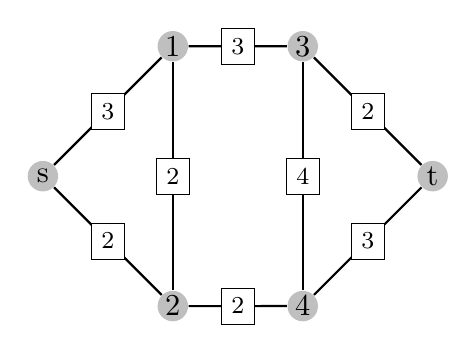
\begin{tikzpicture}[transform shape,label/.style={thin, draw=black, align=center,fill=white,font=\smaller},scale=1.1]
    \node[vertex] (0) at (0,0) {s};
    \node[vertex] (1) at (1.5,1.5) {1};
    \node[vertex] (2) at (1.5,-1.5) {2};
    \node[vertex] (3) at (3,1.5) {3};
    \node[vertex] (4) at (3,-1.5) {4};
    \node[vertex] (5) at (4.5,0) {t};
    \draw[edge] (0) to node[label] {3} (1);
    \draw[edge] (0) to node[label] {2} (2);
    \draw[edge] (1) to node[label] {2} (2);
    \draw[edge] (1) to node[label] {3} (3);
    \draw[edge] (2) to node[label] {2} (4);
    \draw[edge] (3) to node[label] {4} (4);
    \draw[edge] (3) to node[label] {2} (5);
    \draw[edge] (4) to node[label] {3} (5);
  \end{tikzpicture}
  \vspace{10cm}
\end{frame}

\begin{frame}{Finding Paths in Ford Fulkerson -- Problems}

The Ford Fulkerson method does not specify an algorithm for finding a path in the residual graph. You could use anything!\bigskip

\begin{exampleblock}{Problem case with bad path finding}
  The worst case of path selection could be $O(|f^*|E)$, where $f^*$ is the true Max Flow value.\medskip

  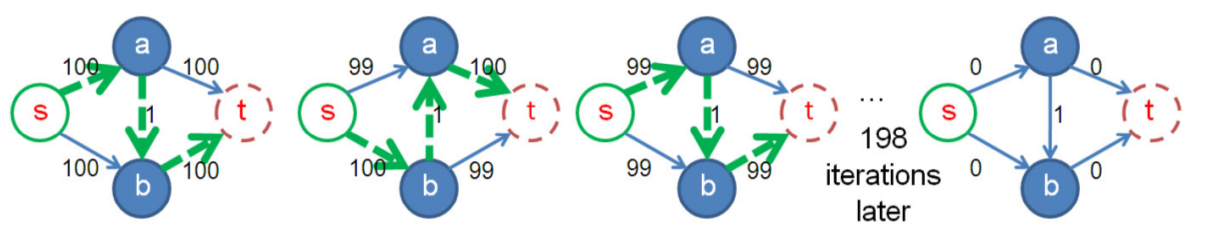
\includegraphics[width=1\textwidth]{../img/ff_worst_halim}
  \ppagenote{Image from "Competitive Programming 3", Steven Halim}
\end{exampleblock}
\end{frame}

\begin{frame}[fragile]
  \frametitle{FF efficient implementation: Edmond Karp's Algorithm}

  \begin{block}{}
    To avoid these "worst cases" of bad path selection, {\bf Edmond Karp}'s algorithm uses BFS on the residual graph to select a new $s\to t$ path.
  \end{block}

{\smaller
\begin{block}{Pseudocode}
\begin{verbatim}
boolean BFS(s, t, p) { } // Finds shortest (by edge #) path from s to t and store in p

mf = 0
while BFS(s,t,p) do {
  for (i in p) {
    minw = min(minw, p[i].w) // find min in p;
  }
  mf += minw;
  for (i in p) {
    res[p[i].u][p[i].v] -= minw;
    res[p[i].v][p[i].u] += minw;
  }
}
\end{verbatim}
\end{block}
}
\end{frame}


\subsection{Maxflow Problem Example}
\begin{frame}
  \frametitle{UVA 259 -- Software Allocation}
    \begin{block}{Outline}
      In a laboratory there are 26 applications and 10 computers. Each computer can run a subset of these applications. Each computer can run only one program per day.\bigskip

      Every day, laboratory users submit {\bf application requests}. These requests can be repeated. For example, two users can request application A, and one user requests application B.

      You must determine if it is possible to satisfy all applications. If so, you must print the computer allocation.
    \end{block}

    \bigskip
    {\bf QUIZ:} How do you solve this program?
\end{frame}

\begin{frame}{UVA -- Software Allocation}

    {\bf Allocation Problems} (also called ``matching''
    problems) can usually be solved using Max Flow.
    \bigskip

    The main part of the problem is: {\bf What is the graph that best represents this problem?}

    \begin{itemize}
      \item Create a {\bf source vertex s} connected to all applications.
      \begin{itemize}
        \item The weight of these edges is the number of users requesting that application.
      \end{itemize}\medskip
      \item Create an edge connecting each application to the computers that can run that application.\medskip
      \item Create an edge connecting each computer to a {\bf sink vertex t}.
      \begin{itemize}
        \item The weight of these edges is 1 (number of programs that can run on the computer).
      \end{itemize}
    \end{itemize}\bigskip

    Solve the maxflow problem for this graph. If the flow size is equal to the number of users, then the allocation is satisfied.
\end{frame}

\begin{frame}{UVA 259 -- Software Allocation}{Input Example One}
A4 01234;\\
Q1 5;\\
P4 56789;\\


   \begin{center}
     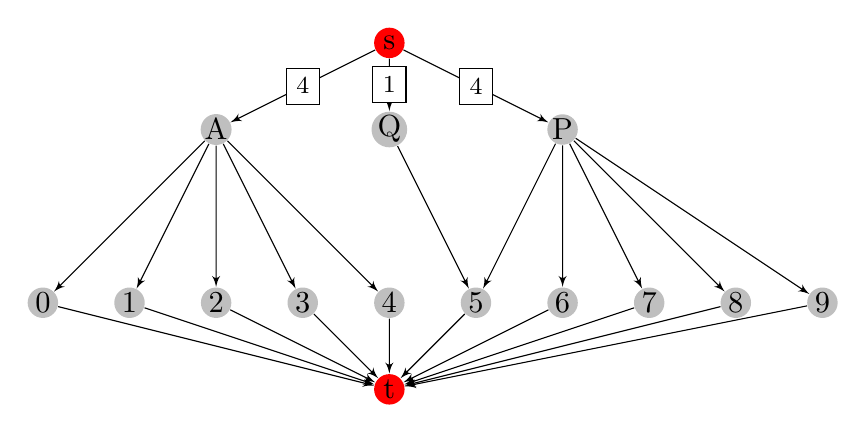
\begin{tikzpicture}[transform shape,label/.style={thin, draw=black, align=center,fill=white,font=\smaller},scale=1.1]
       \tikzset{edge/.style = {->,>=latex'}}
       \node[red vertex] (s) at (0,0) {s};
       \node[vertex] (A) at (-2,-1) {A};
       \node[vertex] (Q) at (0,-1) {Q};
       \node[vertex] (P) at (2,-1) {P};
       \node[vertex] (0) at (-4,-3) {0};
       \node[vertex] (1) at (-3,-3) {1};
       \node[vertex] (2) at (-2,-3) {2};
       \node[vertex] (3) at (-1,-3) {3};
       \node[vertex] (4) at (0,-3) {4};
       \node[vertex] (5) at (1,-3) {5};
       \node[vertex] (6) at (2,-3) {6};
       \node[vertex] (7) at (3,-3) {7};
       \node[vertex] (8) at (4,-3) {8};
       \node[vertex] (9) at (5,-3) {9};
       \node[red vertex] (t) at (0,-4) {t};
       \draw[edge] (s) -- node[label] {4} (A);
       \draw[edge] (s) -- node[label] {1} (Q);
       \draw[edge] (s) -- node[label] {4} (P);
       \draw[edge] (A) -- (0);
       \draw[edge] (A) -- (1);
       \draw[edge] (A) -- (2);
       \draw[edge] (A) -- (3);
       \draw[edge] (A) -- (4);
       \draw[edge] (Q) -- (5);
       \draw[edge] (P) -- (5);
       \draw[edge] (P) -- (6);
       \draw[edge] (P) -- (7);
       \draw[edge] (P) -- (8);
       \draw[edge] (P) -- (9);
       \draw[edge] (0) -- (t);
       \draw[edge] (1) -- (t);
       \draw[edge] (2) -- (t);
       \draw[edge] (3) -- (t);
       \draw[edge] (4) -- (t);
       \draw[edge] (5) -- (t);
       \draw[edge] (6) -- (t);
       \draw[edge] (7) -- (t);
       \draw[edge] (8) -- (t);
       \draw[edge] (9) -- (t);
     \end{tikzpicture}
   \end{center}
\end{frame}

\begin{frame}{UVA 259 -- Software Allocation}{Input Example Two}

A3 0123;\\
B3 1234;\\
 \begin{center}
   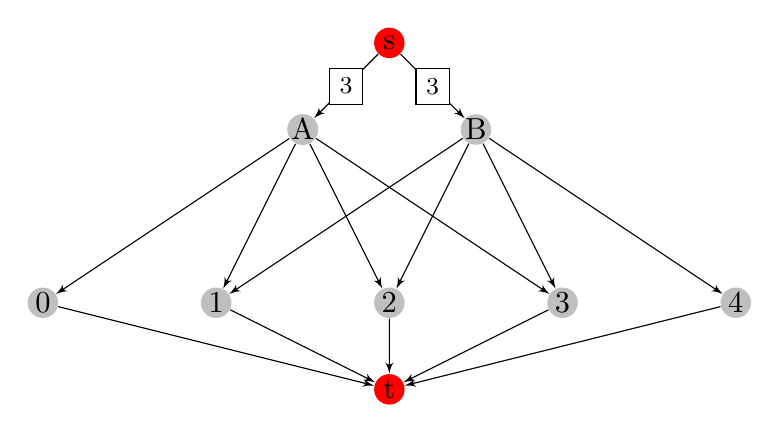
\begin{tikzpicture}[transform shape,label/.style={thin, draw=black, align=center,fill=white,font=\smaller},scale=1.1]
     \tikzset{edge/.style = {->,>=latex'}}
     \node[red vertex] (s) at (0,0) {s};
     \node[vertex] (A) at (-1,-1) {A};
     \node[vertex] (B) at (1,-1) {B};
     \node[vertex] (0) at (-4,-3) {0};
     \node[vertex] (1) at (-2,-3) {1};
     \node[vertex] (2) at (0,-3) {2};
     \node[vertex] (3) at (2,-3) {3};
     \node[vertex] (4) at (4,-3) {4};
     \node[red vertex] (t) at (0,-4) {t};
     \draw[edge] (s) -- node[label] {3} (A);
     \draw[edge] (s) -- node[label] {3} (B);
     \draw[edge] (A) -- (0);
     \draw[edge] (A) -- (1);
     \draw[edge] (A) -- (2);
     \draw[edge] (A) -- (3);
     \draw[edge] (B) -- (1);
     \draw[edge] (B) -- (2);
     \draw[edge] (B) -- (3);
     \draw[edge] (B) -- (4);
     \draw[edge] (0) -- (t);
     \draw[edge] (1) -- (t);
     \draw[edge] (2) -- (t);
     \draw[edge] (3) -- (t);
     \draw[edge] (4) -- (t);
   \end{tikzpicture}
 \end{center}
\end{frame}

\begin{frame}
  \frametitle{UVA 10480 -- Sabotage}
  \begin{block}{Problem Description}
    Given a communication network $V$, what is the {\bf minimum number of edges} that you must remove from $V$ so that the vertices $v_s$ and $v_t$ are not connected?
  \end{block}\bigskip

  This is a traditional graph problem called {\bf minimum cut}. One way to solve this problem is to use the MaxFlow algorithm and analyse the {\bf residual graph}.\bigskip

  \begin{itemize}
    \item After MaxFlow, all edges in the residual graph that have weight $0$ belong to the {\bf minimum cut set}.
    \item A BFS on the residual graph starting from $v_s$ will indicate the vertices that remain connected to $v_s$ after the cut.
    \item The vertices not reachable in the BFS will be connected to $v_e$.
  \end{itemize}
\end{frame}

%% TODO: Add example problems for these cases
\begin{frame}{Designing Network Flow Problem Graphs}
  \begin{block}{Graph with multiple sources and multiple sinks}
  \begin{itemize}
  \item Create a ``super source'' vertex $v_{ss}$. $v_{ss}$ connects to all sources with infinite weight;
  \item Create a ``super sink'' vertex $v_{se}$. All sinks connect to $v_{se}$ with infinite weight;
  \end{itemize}
  \end{block}


  \begin{block}{Graph with weights on vertices, not edges}
    \begin{itemize}
    \item Similar to "full tank", we split the graph's vertices;
    \item Vertex $v_i$ is split into $v_{i1}$ and $v_{i2}$.
    \item Add an edge$(v_{i1}, v_{i2})$ with weight $v_i$.
    \item Don't forget that this solution doubles $|V|$ and increases $|E|$.
    \end{itemize}
  \end{block}
\end{frame}

% \section{Graph Problem Examples}
%
% \begin{frame}{A few more Graph problem example}
%
%   One interesting thing about graph problems is that they come in great variety.\bigskip
%
%   \begin{itemize}
%     \item Many different graph algorithms;
%     \item Many different ways to represent a problem as a graph;
%     \item Many different problem types;
%   \end{itemize}\bigskip
%
%   Let's see some extra problems to discuss these variations.
% \end{frame}
%
% \begin{frame}{Fishmonger -- Shortest path on a DAG}
%   \begin{block}{Problem Description}
%     A fish seller must go from city $v_0$ to city $v_{n-1}$, before the time $t$. The seller must also pay the minimum ammount of toll.\bigskip
%
%     \begin{itemize}
%       \item Every edge has a {\bf toll cost} and a {\bf time cost};
%       \item The number of cities is $\leq 50$, and the time $t$ is $\leq 1000$.
%     \end{itemize}
%   \end{block}\bigskip
%
%   This is a $SSSP$ problem, but with two costs: \emph{time} and \emph{toll}.\medskip
%
%   {\bf Quiz}: How do you find the minimal path for both costs?
% \end{frame}
%
% \begin{frame}
%   \frametitle{Fishmonger -- Shortest path on a DAG}
%
%   \begin{block}{Graph Transformation}
%     Similar to "full tank", we each vertex $v_i$ into $t$ new vertices, where $v_{i,t}$ indicates that you reached vertice $v_{i}$ with $t$ time left.\bigskip
%
%     Each edge is modified: The edges no longer have a time cost, but they instead directionally connect $v_{i,t} \to v_{j,t'}$.
%   \end{block}
%
%   \begin{itemize}
%     \item This transformation multiplies the number of nodes to ($V\times T$);
%     \item However, the new graph is now a DAG;
%     \item Because the graph is a DAG, it is possible to solve the search using {\bf Top-Down Dynamic Programming}:
%     \begin{itemize}
%       \item Recursive function: \emph{find(v,t)}, finds minimum cost $c$
%       \item Table size: $V\times T$
%     \end{itemize}
%     \item In fact, it is not even necessary to \emph{explicitely} transform the graph. An implicit transformation inside the recursive function is enough!
%   \end{itemize}
% \end{frame}
% % TODO: Pseudocode for Fishmonger
%
% \begin{frame}[fragile]
%   \frametitle{Titanic (UVA 11380) -- Network Flow}
%
%   \begin{block}{Problem Outline}
%     Given the map of an accident, calculate how many people escape.
%   \end{block}
%
% \begin{verbatim}
% Map explanation:
% # -- large wood: safe, P people can escape;
% @ -- large iceberg: anyone can pass;
% . -- ice: breaks after 1 person pass;
% * -- initial position: 1 person. Breaks like ice;
% ~ -- freezing water: no one can pass;
% \end{verbatim}
%
%   \begin{center}
%     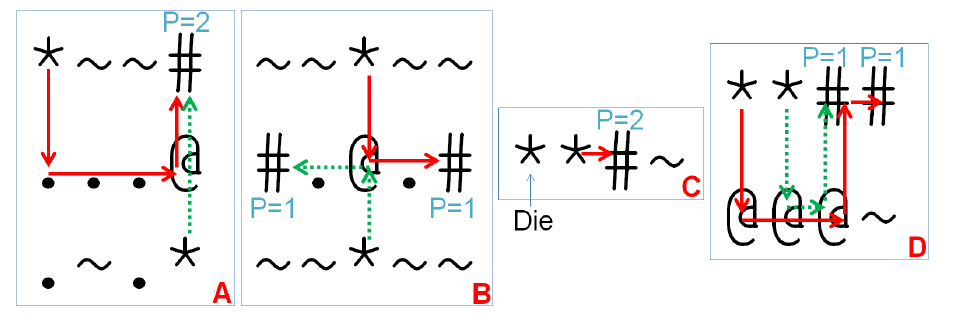
\includegraphics[width=0.7\textwidth]{../img/uva11380_halim}
%   \end{center}
%   \ppagenote{Image from \emph{Competitive Programming, 3rd edition}}
% \end{frame}
%
% \begin{frame}
%   \frametitle{Titanic (UVA11380) -- Network Flow}
%   \begin{block}{Graph Modeling}
%     Number of escaped people = Max Flow of the graph. But how do we create the flow graph?
%   \end{block}
%   One example:
%   \begin{itemize}
%     \item Every non-water cell has two vertices: "In" and "Out";
%     \item Connect "In" and "Out" vertices with cell capacity:
%     \begin{itemize}
%       \item Iceberg and wood: Infinite
%       \item ice and initial position: 1
%     \end{itemize}
%     \item Connect every "Out" vertex with other nearby "In" vertices with infinite capacity;
%     \item Connect "Super Source" with all "initial positions" with capacity 1;
%     \item Connect all "Wood" with "Super Sink", with capacity P.
%   \end{itemize}
% \end{frame}

\begin{frame}
  \frametitle{Prime Pairing -- Bipartite Graph Flow}
  \begin{block}{Problem Description}
    Two numbers $a,b$ are be {\bf prime paired} if $a+b$ is prime.\bigskip

    Given a set of numbers $N$, is it possible to create a {\bf complete pairing} with all elements of $N$?
  \end{block}\bigskip

  Example:
  \begin{itemize}
  \item $N = \{1,4,7,10,11,12\}$
  \item Pairing: $\{1,4\}, \{7,10\}, \{11,12\}$
  \end{itemize}

  \vfill

  Is this even a graph problem??
\end{frame}

\begin{frame}
  \frametitle{Prime Pairing -- Bipartite Graph Flow}
  \begin{block}{Trick}
    It is possible to think of this problem as an {\bf allocation} problem.\bigskip

    Remember that {\bf even + even = even} and {\bf odd + odd = even}. So a prime pair must be one even \# and one odd \#.\bigskip

    In this way, we must allocate even numbers to odd numbers (or vice-versa)
  \end{block}

  How to create the graph:
  \begin{itemize}
  \item Split set between odds and evens;
  \item If \#odd is not equal to \#even, there is no solution;
  \item Create edges between odds and evens if they are a prime pair;
  \item Add a super source and super sink;
  \end{itemize}\bigskip

  If max flow = \# vertices / 2, then there is a solution.
\end{frame}

%\begin{frame}
%  \frametitle{Flow and Special Graph problems}
% %% TODO: Add more special problems from the book for discussion
%\end{frame}

\section{Conclusion}

\begin{frame}
  \frametitle{Lecture Summary}

  Graph Algorithms for Path Finding and Maximum Flow:\bigskip

  \begin{itemize}
    \item Single Source Shortest Path:
    \begin{itemize}
      \item In an unweighted graph, use BFS;
      \item For a weighted graph, use Dijkstra;
      \item If the graph has negative loops, Bellman-ford will terminate;
    \end{itemize}\medskip
    \item All Pairs Shortest path:
    \begin{itemize}
      \item Floyd-Warshall is very easy to program, but costs $O(V^3)$;
      \item You could also just repeat Dijkstra $V$ times;
    \end{itemize}\medskip
    \item Maximum Flow:
    \begin{itemize}
      \item The Ford-Fergusson Method describes how to find the maximum Flow;
      \item Edmond-Karp implements FF using BFS on the residual graph to find minimum paths;
    \end{itemize}
  \end{itemize}\bigskip

  The most important skill to learn for graph problems is {\bf how to transform the problem graph}.
\end{frame}


% \subsection{Problem Discussion}
%
% \begin{frame}
%   \frametitle{This Week's Problems}
%   \begin{itemize}
%   \item Wormholes;
%   \item Meeting Professor Miguel;
%   \item Full Tank?;
%   \item Degrees of Separation;
%   \item Avoiding your Boss;
%   \item Software Allocation;
%   \item Sabotage;
%   \item Gopher II;
%   \end{itemize}
% \end{frame}
%
% \begin{frame}
%   \frametitle{Problem Hints}
%   \begin{block}{Wormholes}
%     \begin{itemize}
%     \item {\bf Problem goal:} Find a negative weight loop in the graph
%     \item {\bf Hint:} Just follow the suggestions from the class
%     \end{itemize}
%   \end{block}
%
%   \begin{exampleblock}{Meeting Professor Miguel}
%     \begin{itemize}
%     \item {\bf Problem goal:} Find the shortest path from the student to the professor.
%     \item {\bf Trick:} Some edges only the student can walk, some
%       edges only the professor can walk;
%     \item {\bf Hint 1:} There are really two graphs: One for the student, one for the
%       professor;
%     \item {\bf Hint 2:} The graphs are really small;
%     \end{itemize}
%   \end{exampleblock}
% \end{frame}
%
% \begin{frame}
%   \frametitle{Problem Hints}
%   \begin{block}{Full Tank?}
%     \begin{itemize}
%     \item Discussed in class;
%     \item Good practice on modifying graphs to solve problems;
%     \end{itemize}
%   \end{block}
%   \begin{exampleblock}{Degrees of Separation}
%     \begin{itemize}
%     \item {\bf Problem Outline:} Given a network of relationship, define the "Degree of Separation" of the network. "Degree of separation" is the {\bf largest shortest path} in the network.\bigskip
%
%     \item {\bf Hint 1:} Don't forget the special case of a disconnected Graph;
%     \item {\bf Hint 2:} The "largest shortest path" of a graph is also known as the {\bf diameter}, and it is an important property of graphs;
%     \end{itemize}
%   \end{exampleblock}
% \end{frame}
%
% \begin{frame}
%   \frametitle{Problem Hints}
%   \begin{block}{Avoiding Your Boss}
%     \begin{itemize}
%     \item {\bf Problem Goal:} You are going from your house to the market. Your boss is going from her house to the office. Can you find a path that does not meet your boss' path?\bigskip
%
%     \item {\bf Hint:} How do you modify the graph so that you can avoid your boss?
%     \end{itemize}
%   \end{block}
%
%   \begin{exampleblock}{Software Allocation}
%     \begin{itemize}
%     \item Discussed in Class;
%     \item Use this problem to practice "Max Flow";
%     \end{itemize}
%   \end{exampleblock}
% \end{frame}
%
% \begin{frame}
%   \frametitle{Problem Hints}
%   \begin{block}{Sabotage}
%     \begin{itemize}
%     \item {\bf Problem Goal:} Find the cost of minimum cut;
%     \item Discussed in class, use Max Flow to find the minimum cut set;
%     \end{itemize}
%   \end{block}
%
%   \begin{exampleblock}{Gopher II}
%     {\bf Problem Outline:}
%     \begin{itemize}
%     \item You receive the position of $N$ gophers and $M$ gopher holes.
%     \item Each hole can save 1 Gopher, Gophers run at speed $v$.
%     \item Hawks will eat the Gophers after $t$ seconds;
%     \item How many gophers are saved? How many are eatern?
%     \end{itemize}
%     {\bf Hints}:
%     \begin{itemize}
%       \item Think of an {\bf Allocation} of gophers to holes;
%       \item Graph is implicit: How do you define the edges?
%     \end{itemize}
%   \end{exampleblock}
% \end{frame}


%%%%%%%%%%%%%%%%%%%%%%%%%%%%%%%%%%%%%%%%%%%%%%%%%%%%
\section{Backmatter}
\begin{frame}{About these Slides}
  These slides were made by Claus Aranha, 2020. You are welcome to copy, re-use and modify this material.
  \bigskip

  Individual images in some slides might have been made by other
  authors. Please see the references in each slide for those cases.
\end{frame}

\begin{frame}[allowframebreaks]{Image Credits}
  \printnotes
\end{frame}

\end{CJK}
\end{document}
